\chapter{Batch Python Scripting}
\label{chap:BatchPythonScripting}

Python scripting can be leveraged in two ways within ParaView.  First,
Python scripts can automate the setup and execution of visualizations by
performing the same actions as a user at the GUI.  Second, Python scripts
can be run inside pipeline objects, thereby performing parallel
visualization algorithms.  This chapter describes the first mode, batch
scripting for automating the visualization.

Batch scripting is a good way to automate mundane or repetitive tasks, but
it is also a critical component when using ParaView in situations where the
GUI is undesired or unavailable.  The automation of Python scripts allows
you to leverage ParaView as a scalable parallel post-processing framework.
We are also leveraging Python scripting to establish \emph{in-situ}
computation within simulation code (a.k.a. co-processing).

This tutorial gives only a brief introduction to Python scripting.  The
most recent and complete documentation is kept on the ParaView Wiki.

\begin{quote}
  \href{http://www.paraview.org/Wiki/ParaView/Python_Scripting}{http://www.paraview.org/Wiki/ParaView/Python\_Scripting}
\end{quote}

\section{Starting the Python Interpreter}
\label{sec:StartingThePythonInterpreter}

There are many ways to invoke the Python interpreter.  The method you use
depends on how you are using the scripting.  The easiest way to get a
python interpreter, and the method we use in this tutorial, is to select
\gui{Tools} \ra \gui{Python Shell} from the menu.  This will bring up a
dialog box containing controls for ParaView's python shell. The left
hand side of the dialog is a Python interpreter, where you directly control
ParaView via the interface described below. On the right hand side are
controls for saving and loading python scripts on disk, for managing
\keyterm{macros} which are scripts that are accesible directly from
ParaView's main menu bar, and for recording \keyterm{traces}, which
are scripts that reproduce the actions initiated via ParaView's
normal GUI interface.

\begin{inlinefig}
  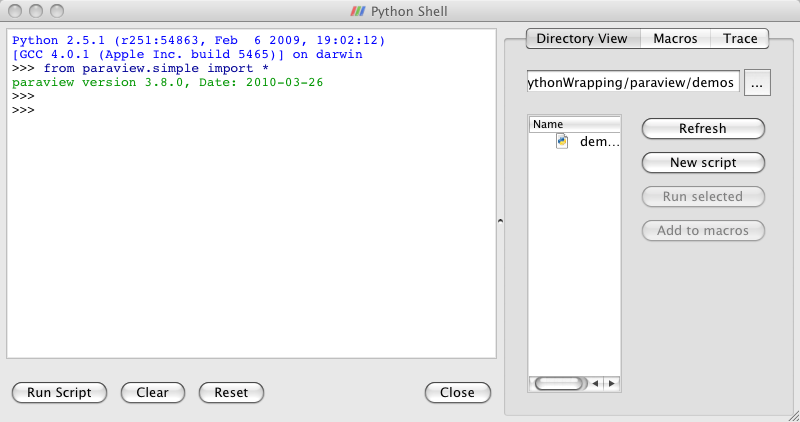
\includegraphics[width=4in]{images/PythonShellDialog}
\end{inlinefig}

If you are right now most interested in getting started on writing scripts,
feel free to skip to the next section past the discussion of the other ways
to invoke scripting.

ParaView comes with two command line programs that execute Python scripts:
\commandline{pvpython} and \commandline{pvbatch}.  They are similar to the
\commandline{python} executable that comes with Python distributions in
that they accept Python scripts either from the command line or from a file
and they feed the scripts to the Python interpreter.

The difference between \commandline{pvpython} and \commandline{pvbatch} is
subtle and has to do with the way they establish the visualization
service.  \commandline{pvpython} is roughly equivalent to the
\commandline{paraview} client GUI with the GUI replaced with the Python
interpreter.  It is a serial application that connects to a ParaView server
(which can be either builtin or remote).  \commandline{pvbatch} is roughly
equivalent to \commandline{pvserver} except that commands are taken from a
Python script rather than from a socket connection to a client.  It is a
parallel application that can be launched with \commandline{mpirun} (assuming
it was compiled with MPI), but it cannot connect to another server; it is
its own server.  In general, you should use \commandline{pvpython} if you
will be using the interpreter interactively and \commandline{pvbatch} if
you are running in parallel.

It is also possible to use the ParaView Python modules from programs
outside of ParaView.  This can be done by pointing the \texttt{PYTHONPATH}
environment variable to the location of the ParaView libraries and Python
modules and pointing the \texttt{LD\_LIBRARY\_PATH} (on Unix/Linux/Mac) or
\texttt{PATH} (on Windows) environment variable to the ParaView libraries.
Running the Python script this way allows you to take advantage of
third-party applications such as IDLE.  For more information on setting up
your environment, consult the ParaView Wiki.

\section{Creating a Pipeline}
\label{sec:CreatingAPipeline}

We should first note that the ParaView GUI's python \gui{Trace} feature
allows one to very easily create Python scripts for many common
tasks. To use \gui{Trace}, one simply begins a trace recording via the GUI's
\gui{Python Shell} dialog, uses the ParaView GUI to construct a
visualization, and then stops the trace recording. This produces a
python script that reconstructs the actions taken in the GUI. That
script contains exactly the same set of operations that we are
about to describe. As such, \gui{Trace} recordings are a good resource when
you are trying to figure out how to do some action via the python
interface, and conversely the following descriptions will help in
understanding the contents of any given \gui{Trace} script.

The first thing any ParaView Python script must do is load the
\textpy{paraview.simple} module.  This is done by invoking
\begin{python}
from paraview.simple import *
\end{python}
In general, this command needs to be invoked at the beginning of any
ParaView batch Python script.  This command is automatically invoked for
you when you bring up the scripting dialog in ParaView, but you must add it
yourself when using the Python interpreter in other programs (including
\commandline{pvpython} and \commandline{pvbatch}).

The \textpy{paraview.simple} module defines a function for every source,
reader, filter, and writer defined in ParaView.  The function will be the
same name as shown in the GUI menus with spaces and special characters
removed.  For example, the \pyfunc{Sphere} function corresponds to
\gui{Sources} \ra \gui{Sphere} in the GUI and the \pyfunc{PlotOverLine}
function corresponds to \gui{Filters} \ra \gui{Data Analysis} \ra \gui{Plot
  Over Line}.  Each function creates a pipeline object, which will show up
in the pipeline browser (with the exception of writers), and returns an
object that is a proxy that can be used to query and manipulate the
properties of that pipeline object.

There are also several other functions in the \textpy{paraview.simple}
module that perform other manipulations.  For example, the pair of
functions \pyfunc{Show} and \pyfunc{Hide} turn on and off, respectively,
the visibility of a pipeline object in a view.  The \pyfunc{Render}
function causes a view to be redrawn.

\begin{exercise}{Creating and Showing a Source}
  \label{ex:CreatingAndShowingASource}%
  If you have been following an exercise in a previous section, now is a
  good time to reset ParaView.  The easiest way to do this is to press
  the~\disconnect button.

  If you have not already done so, open the Python shell in the ParaView
  GUI by selecting \gui{Tools} \ra \gui{Python Shell} from the menu.  You
  will notice that
  \begin{python}
from paraview.simple import *
  \end{python}
  has been added for you.

  Create and show a \gui{Sphere} source by typing the following in the
  Python shell.
  \begin{python}
sphere = Sphere()
Show()
Render()
  \end{python}

  The \pyfunc{Sphere} command creates a sphere pipeline object.  Once it is
  executed you will see an item in the pipeline browser created.  We save a
  proxy to the pipeline object in the variable \textpy{sphere}.  We are
  not using this variable (yet), but it is good practice to save references
  to your pipeline objects.

  The subsequent \pyfunc{Show} command turns on visibility of this object in
  the view, and the subsequent \pyfunc{Render} causes the results to be
  seen.  At this point you can interact directly with the GUI again.  Try
  changing the camera angle in the view with the mouse.
\end{exercise}

\begin{exercise}{Creating and Showing a Filter}
  \label{ex:CreatingAndShowingAFilter}%
  Creating filters is almost identical to creating sources.  By default,
  the last created pipeline object will be set as the input to the newly
  created filter, much like when creating filters in the GUI.

  This exercise is a continuation of
  Exercise~\ref{ex:CreatingAndShowingASource}.  You will need to finish
  that exercise before beginning this one.

  Type in the following script in the Python shell that hides the sphere
  and then adds the shrink filter to the sphere and shows that.

  \pyfuncindex{Hide}\pyfuncindex{Show}\pyfuncindex{Shrink}\pyfuncindex{Render}
  \begin{python}
Hide()
shrink = Shrink()
Show()
Render()
  \end{python}

  The sphere should be replaced with the output of the \pyfunc{Shrink}
  filter, which makes all of the polygons smaller to give the mesh an
  exploded type of appearance.
\end{exercise}

So far as we have built pipelines we have accepted the default parameters
for the pipeline objects.  As we have seen in the exercises of
Chapter~\ref{chap:BasicUsage}, it is common to have to modify the
parameters of the objects using the object inspector.

In Python scripting, we use the proxy returned from the creation functions
to manipulate the pipeline objects.  These proxies are in fact Python
objects with class attributes that correspond to the same properties you
set in the Object Inspector.  They have the same names as those in the
object inspector with spaces and other illegal characters removed.  You can
set them by simply assigning them a value.

\begin{exercise}{Changing Pipeline Object Properties}
  \label{ex:ChangingPipelineObjectProperties}%
  This exercise is a continuation of Exercises
  \ref{ex:CreatingAndShowingASource} and
  \ref{ex:CreatingAndShowingAFilter}.  You will need to finish those
  exercises before beginning this one.

  Recall that we have so far created two Python variables, \textpy{sphere}
  and \textpy{shrink}, that are proxies to the corresponding pipeline
  objects.  First, enter the following command into the Python shell to get
  the current value of the \gui{Theta Resolution} property of the sphere.

  \begin{python}
print sphere.ThetaResolution
  \end{python}

  The Python interpreter should respond with the result \textpy{8}.  (Note
  that using the \textpy{print} keyword, which instructs Python to output
  the arguments to standard out, is superfluous here as the Python shell
  will output the result of any command anyway.)  Let us double the number
  of polygons around the equator of the sphere by changing this property.

  \begin{python}
sphere.ThetaResolution = 16
Render()
  \end{python}

  The shrink filter has only one property, \gui{Shrink Factor}.  We can
  adjust this factor to make the size of the polygons larger or smaller.
  Let us change the factor to make the polygons smaller.

  \begin{python}
shrink.ShrinkFactor = 0.25
Render()
  \end{python}

  You may have noticed that as you type in Python commands to change the
  pipeline object properties, the GUI in the object inspector updates
  accordingly.
\end{exercise}

So far we have created only non-branching pipelines.  This is a simple and
common case and, like many other things in the \textpy{paraview.simple}
module, is designed to minimize the amount of work for the simple and
common case but also provide a clear path to the more complicated cases.
As we have built the non-branching pipeline, ParaView has automatically
connected the filter input to the previously created object so that the
script reads like the sequence of operations it is.  However, if the
pipeline has branching, we need to be more specific about the filter
inputs.

\begin{exercise}{Branching Pipelines}
  \label{ex:BranchingPipelines}%
  This exercise is a continuation of Exercises
  \ref{ex:CreatingAndShowingASource} through
  \ref{ex:ChangingPipelineObjectProperties}.  You will need to finish
  Exercises \ref{ex:CreatingAndShowingASource} and
  \ref{ex:CreatingAndShowingAFilter} before beginning this one
  (Exercise~\ref{ex:ChangingPipelineObjectProperties} is optional).

  Recall that we have so far created two Python variables, \textpy{sphere}
  and \textpy{shrink}, that are proxies to the corresponding pipeline
  objects.  We will now add a second filter to the sphere source that will
  extract the wireframe from it.  Enter the following in the Python shell.

  \pyfuncindex{ExtractEdges}
  \begin{python}
wireframe = ExtractEdges(Input=sphere)
Show()
Render()
  \end{python}

  An \gui{Extract Edges} filter is added to the sphere source.  You should
  now see both the wireframe of the original sphere and the shrunken
  polygons.

  Notice that we explicitly set the input for the \gui{Extract Edges}
  filter by providing \textpy{Input=sphere} as an argument to the
  \pyfunc{ExtractEdges} function.  What we are really doing is setting the
  \textpy{Input} property upon construction of the object.  Although it
  would be possible to create the object with the default input, and then
  set the input later, it is not recommended.  The problem is that not all
  filters accept all input.  If you initially create a filter with the
  wrong input, you could get error messages before you get a chance to
  change the \textpy{Input} property to the correct input.

  The sphere source having two filters connected to its output is an
  example of \keyterm{fan out} in the pipeline.  It is always possible to
  have multiple filters attached to a single output.  Some filters, but not
  all, also support having multiple filters connected to their input.
  Multiple filters are attached to an input is known as \keyterm{fan in}.
  In ParaView's Python scripting, fan in is handled much like fan out, by
  explicitly defining a filter's inputs.  When setting multiple inputs (on
  a single port), simply set the input to a list of pipeline objects rather
  than a single one.  For example, let us group the results of the shrink
  and extract edges filters using the \gui{Group Datasets} filter.  Type
  the following line in the Python shell.

  \pyfuncindex{GroupDatasets}
  \begin{python}
group = GroupDatasets(Input=[shrink,wireframe])
Show()
  \end{python}

  There is now no longer any reason for showing the shrink and extract
  edges filters, so let us hide them.  By default, the \pyfunc{Show} and
  \pyfunc{Hide} functions operate on the last pipeline object created (much
  like the default input when creating a filter), but you can explicitly
  choose the object by giving it as an argument.  To hide the shrink and
  extract edges filters, type the following in the Python shell.

  \begin{python}
Hide(shrink)
Hide(wireframe)
Render()
  \end{python}
\end{exercise}

In the previous exercise, we saw that we could set the \textpy{Input}
property by placing \textpy{Input=\argdesc{input object}} in the arguments
of the creator function.  In general we can set any of the properties at
object construction by specifying \textpy{\argdesc{property
    name}=\argdesc{property value}}.  For example, we can set both the
\gui{Theta Resolution} and \gui{Phi Resolution} when we create a sphere
with a line like this.

\begin{python}
sphere = Sphere(ThetaResolution=360, PhiResolution=180)
\end{python}


\section{Active Objects}
\label{sec:ActiveObjects}

If you have any experience with the ParaView GUI, then you should already
be familiar with the concept of an active object.  As you build and
manipulate visualizations within the GUI, you first have to select an
object in the pipeline browser.  Other GUI panels such as the object
inspector will change based on what the active object is.  The active
object is also used as the default object to use for some operations such
as adding a filter.

The batch Python scripting also understands the concept of the active
object.  In fact, when running together, the GUI and the Python interpreter
share the same active object.  When you created filters in the previous
section, the default input they were given was actually the active object.
When you created a new pipeline object, that new object became the active
one (just like when you create an object in the GUI).

You can get and set the active object with the \pyfunc{GetActiveSource} and
\pyfunc{SetActiveSource} functions, respectively.  You can also get a list
of all pipeline objects with the \pyfunc{GetSources} function.  When you
click on a new object in the GUI pipeline browser, the active object in
Python will change.  Likewise, if you call \pyfunc{SetActiveSource} in
python, you will see the corresponding entry become highlighted in the
pipeline browser.

\begin{exercise}{Experiment with Active Pipeline Objects}
  \label{ex:ExperimentWithActivePipelineObjects}%
  This exercise is a continuation of the exercises in the previous
  section.  However, if you prefer you can create any pipeline you want and
  follow along.

  Play with active objects by trying the following.
  \begin{itemize}
  \item Get a list of objects by calling
    \pyfuncindex{GetSources}\textpy{GetSources()}.  Find the sources and
    filters you created in that list.
  \item Get the active object by calling
    \pyfuncindex{GetActiveSource}\textpy{GetActiveSource()}.  Compare that
    to what is selected in the pipeline browser.
  \item Select something new in the pipeline browser and call
    \textpy{GetActiveSource()} again.
  \item Change the active object with the \pyfunc{SetActiveSource}
    function.  Observe the change in the pipeline browser.
  \end{itemize}
\end{exercise}

In addition to maintaining an active pipeline object, ParaView Python
scripting also maintains an active view.  As a ParaView user, you should
also already be familiar with multiple views and the active view.  The
active view is marked in the GUI with a blue border.  The Python functions
\pyfunc{GetActiveView} and \pyfunc{SetActiveView} allow you to query and
change the active view.  As with pipeline objects, the active view is
synchronized between the GUI and the Python interpreter.


\section{Online Help}
\label{sec:OnlineHelp}

This tutorial, as well as similar instructions in the ParaView book and
Wiki, is designed to give the key concepts necessary to understand and
create batch Python scripts.  The detailed documentation including complete lists of
functions, classes, and properties available is maintained by the ParaView
build process and provided as online help from within the ParaView
application.  In this way we can ensure that the documentation is up to
date for whatever version of ParaView you are using and that it is easily
accessible.

The ParaView Python bindings make use of the \pyfunc{help} built-in
function.  This function takes as an argument any Python object and returns
some documentation on it.  For example, typing
\begin{python}
  help(paraview.simple)
\end{python}
returns a brief description of the module and then a list of all the
functions included in the module with a brief synopsis of what each one
does.  For example
\begin{python}
  help(Sphere)
  sphere = Sphere()
  help(sphere)
\end{python}
will first give help on the \pyfunc{Sphere} function, then use it to create
an object, and then give help on the object that was returned (including a
list of all the properties for the proxy).

Most of the panels displayed in the object inspector's \gui{Properties} tab
are automatically generated from the same introspection that builds the
Python classes. (There are a small number of exceptions where a custom
panel was created for better usability.) Thus, if you see a labeled widget
in the object inspector, there is a good chance that there is a
corresponding property in the Python object with the same name.

Regardless of whether the GUI contains a custom panel for a pipeline
object, you can still get information about that object's properties from
the GUI's online help.  As always, bring up the help with the
\icon{pqHelp32} toolbar button.  You can find documentation for all the
available pipeline objects under the \gui{Sources Menu}, \gui{Filters
  Menu}, \gui{Readers}, and \gui{Writers} entries in the help
\gui{Contents}.  Each entry gives a list of objects of that type.  Clicking
on any one of the objects gives a list of the properties you can set from
within Python.

\begin{inlinefig}
  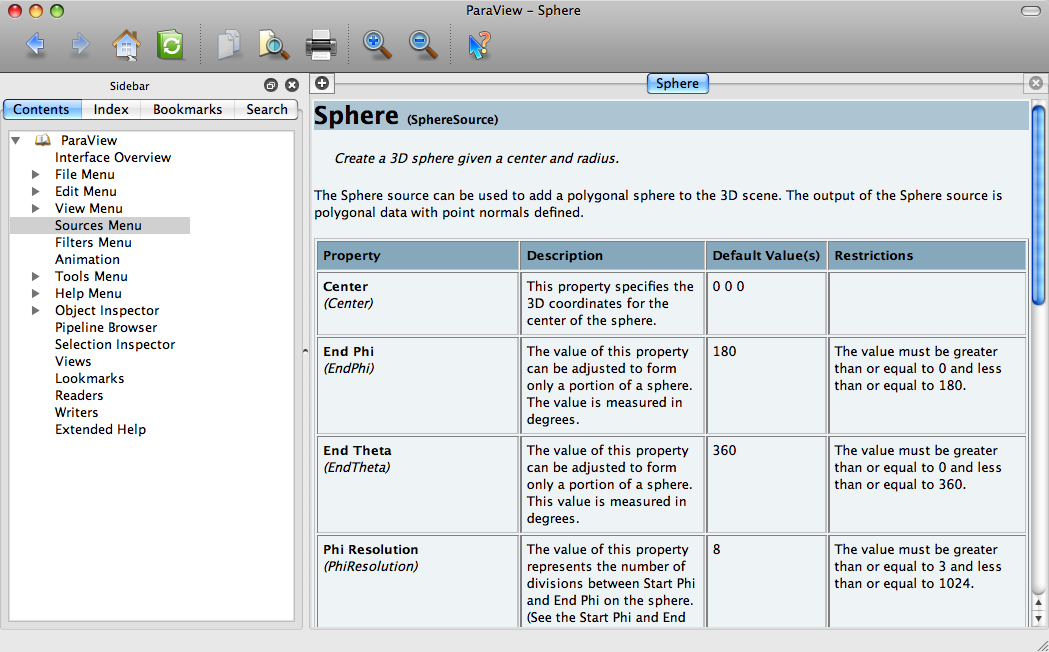
\includegraphics[width=3in]{images/ObjectHelp}
\end{inlinefig}


\section{Reading from Files}
\label{sec:ReadingFromFiles}

The equivalent to opening a file in the ParaView GUI is to create a reader
in Python scripting.  Reader objects are created in much the same way as
sources and filters; \textpy{paraview.simple} has a function for each
reader type that creates the pipeline object and returns a proxy
object. One can instantatiate any given reader directly as described
below, or more simply call \textpy{reader = OpenDataFile(\argdesc{filename})}

All reader objects have at least one property (hidden in the GUI) that
specifies the file name.  This property is conventionally called either
\textpy{FileName} or \textpy{FileNames}.  You should always specify a valid
file name when creating a reader by placing something like
\textpy{FileName=\argdesc{full path}} in the arguments of the construction
object.  Readers often do not initialize correctly if not given a valid
file name.

\begin{exercise}{Creating a Reader}
  \label{ex:CreatingAReader}%
  We are going to start a fresh visualization, so if you have been
  following along with the exercises so far, now is a good time to reset
  ParaView.  The easiest way to do this is to press the~\disconnect button.
  You will also need the Python shell.  If you have not already done so,
  open it with \gui{Tools} \ra \gui{Python Shell} from the menu.

  In this exercise we are loading the \gui{disk\_out\_ref.ex2} file from
  the Python shell.  Locate this file on your computer and be ready to type
  or copy it into the Python shell.  We will reference it as
  \textpy{\argdesc{path}/disk\_out\_ref.ex2}.

  Create the reader while specifying the file name by entering the following
  in the Python shell.

  \begin{pythonpluscommands}
reader = ExodusIIReader(FileName='\argdesc{path}/disk_out_ref.ex2')
Show()
Render()
  \end{pythonpluscommands}
\end{exercise}


\section{Querying Field Attributes}
\label{sec:QueryingFieldAttributes}

In addition to having properties specific to the class, all proxies for
pipeline objects share a set of common properties and methods.  Two very
important such properties are the \pyattrib{PointData} and
\pyattrib{CellData} properties.  These properties act like
\keyterm{dictionaries}, an associative array type in Python, that maps
variable names (in strings) to \pyattrib{ArrayInformation} objects that
hold some characteristics of the fields.  Of particular note are the
\pyattrib{ArrayInformation} methods \pyfunc{GetName}, which returns the
name of the field, \pyfunc{GetNumberOfComponents}, which returns the size
of each field value (1 for scalars, more for vectors), and
\pyfunc{GetRange}, which returns the minimum and maximum values for a
particular component.

\begin{exercise}{Getting Field Information}
  \label{ex:GettingFieldInformation}%
  This exercise is a continuation of Exercise~\ref{ex:CreatingAReader}.
  You will need to finish that exercise before beginning this one.

  To start with, get a handle to the point data and print out all of the
  point fields available.
  \begin{python}
pd = reader.PointData
print pd.keys()
  \end{python}

  Get some information about the ``Pres'' and ``V'' fields.
  \begin{python}
print pd['Pres'].GetNumberOfComponents()
print pd['Pres'].GetRange()
print pd['V'].GetNumberOfComponents()
  \end{python}

  Now let us get fancy.  Use the Python \pyattrib{for} construct to iterate
  over all of the arrays and print the ranges for all the components.
  \begin{python}
for ai in pd.values():
    print ai.GetName(), ai.GetNumberOfComponents(),
    for i in xrange(ai.GetNumberOfComponents()):
        print ai.GetRange(i),
    print
  \end{python}
\end{exercise}


\section{Representations}
\label{sec:Representations}
\index{representation}

Representations are the ``glue'' between the data in a pipeline object and
a view.  The representation is responsible for managing how a data set is
drawn in the view.  The representation defines and manages the underlying
rendering objects used to draw the data as well as other rendering
properties such as coloring and lighting.  Parameters made available in the
\gui{Display} panel of the GUI are managed by representations.  There is a
separate representation object instance for every pipeline-object--view
pair.  This is so that each view can display the data differently.

Representations are created automatically.  You can get the proxy to the
representation objects with the \pyfunc{GetRepresentation} function.  With
no arguments, this function will return the representation for the active
pipeline object and the active view.  You can also specify a pipeline
object or view or both.

\begin{exercise}{Coloring Data}
  \label{ex:ColoringData}%
  This exercise is a continuation of Exercise~\ref{ex:CreatingAReader} (and
  optionally Exercise~\ref{ex:GettingFieldInformation}).  If you do not
  have the exodus file open, you will need to finish that exercise before
  beginning this one.

  Let us change the color of the geometry to blue and give it a very
  pronounced specular highlight (that is, make it really shiny).  Type in
  the following into the Python shell to get the representation and change
  the material properties.

  \begin{python}
readerRep = GetRepresentation()
readerRep.DiffuseColor = [0, 0, 1]
readerRep.SpecularColor = [1, 1, 1]
readerRep.SpecularPower = 128
readerRep.Specular = 1
Render()
  \end{python}

  Now rotate the camera with the mouse in the GUI to see the effect of the
  specular highlighting.

  We can also use the representation to color by a field variable.  Enter
  the following into the Python shell to color the mesh by the ``Pres''
  field variable.

  \begin{python}
readerRep.ColorArrayName = 'Pres'
readerRep.LookupTable = MakeBlueToRedLT(0, 0.03)
Render()
  \end{python}
\end{exercise}

% Chapter Batch Python Scripting
